\documentclass[11pt,a4paper]{article}

% --- Packages ---
\usepackage[utf8]{inputenc}
\usepackage[T1]{fontenc}
\usepackage{lmodern}
\usepackage[margin=1in]{geometry}
\usepackage{amsmath,amssymb,amsfonts}
\usepackage{graphicx}
\usepackage{booktabs}
\usepackage{array}
\usepackage{microtype}
\usepackage{xcolor}
\usepackage{caption}
\usepackage{subcaption}
\usepackage{enumitem}
\usepackage{cite}
\usepackage{hyperref}

\hypersetup{
    colorlinks=true,
    linkcolor=blue!70!black,
    citecolor=blue!70!black,
    urlcolor=blue!70!black
}

\title{\textbf{Multimodal Meme Understanding: Image, Text, or Both?}}

\author{}
\date{October 2026}

\begin{document}

\maketitle

\begin{abstract}
Memes often need both words and pictures to make sense. In this project, we test whether using both inputs helps predict a meme's sentiment: negative, neutral, or positive. We compare a BERT text-only model and a ResNet-50 image-only model with three combined models: concatenation, product, and cross-attention. We test all five models on the same 700 memes using three random seeds. Concatenation gets the highest average macro-F1 at 33.69 percent, compared with 30.94 percent for text and 30.81 percent for images. Cross-attention gets the highest average accuracy among the trained models at 46.76 percent. Concatenation recognizes neutral memes better, but misses more positive memes. However, all fusion-versus-baseline confidence intervals include zero and all adjusted p-values exceed 0.05, so we find no statistically clear gain from combining inputs; fusion mainly shifts predictions toward neutral. Results also vary across sarcasm, humor, and motivation groups. We examine 20 examples where models make mistakes or correct another model's mistake. Removing exact overlaps with training data does not change the leading fusion model. Overall, text and images help on different examples, but combining them does not improve every prediction or prove that a model understands the joke.

\end{abstract}
\section{Introduction and Research Questions}
\label{sec:intro}

A meme can mean something different when we look at its text and image together. A positive sentence may become sarcastic when it appears beside an annoyed face. Some jokes also depend on a familiar character, scene, or meme template. This makes sentiment prediction harder than simply looking for positive or negative words. Our project studies one part of meme understanding: predicting whether the overall sentiment is negative, neutral, or positive. We do not test whether a model can explain a joke or recognize every cultural reference.

BERT~\cite{devlin2019bert} uses the caption, while ResNet-50~\cite{he2016deep} uses the image. Each input may contain useful information that the other misses. However, image-only still includes words printed inside the picture. Combining both inputs does not always improve results~\cite{bonheme2020sesam}. We compare actual predictions rather than assume that using both inputs must be better. The Memotion data~\cite{sharma2020semeval} also has practical problems, such as damaged images, imperfect captions, and many more positive examples than negative ones.

We test the models with three random seeds to answer these questions:
\begin{itemize}[leftmargin=*,itemsep=1pt,topsep=2pt]
\item \textbf{RQ1 (Image or text):} How well do the image-only and text-only models predict sentiment? Is one consistently better?
\item \textbf{RQ2 (Using both):} Does combining text and images improve the scores, and is the improvement supported by statistical tests?
\item \textbf{RQ3 (When it helps):} Which sentiment, sarcasm, humor, and motivation groups benefit from combining inputs? Where does it cause mistakes?
\end{itemize}

\paragraph{Our work.} Our group completed three main parts of the project:
\begin{enumerate}[leftmargin=*,itemsep=1pt,topsep=2pt]
\item \textbf{Data preparation:} Checking images, grouping five sentiment labels into three classes, and giving more weight to less common classes during training.
\item \textbf{Model comparison:} Testing BERT, ResNet-50, and three ways of combining their features across three seeds.
\item \textbf{Result and error analysis:} Comparing scores, checking uncertainty, studying meme groups, and examining mistakes. Possible reasons for errors are discussed without treating them as proven causes.
\end{enumerate}

\section{Related Work}
\label{sec:related}

\subsection{Sentiment prediction with several inputs}
Multimodal sentiment analysis uses more than one kind of input, such as text, images, or sound. Tensor Fusion Network~\cite{zadeh2017tensor} combines language, visual, and audio information to predict sentiment in videos. Videos often have speech and facial movements that happen together. Memes are different: a single picture and caption may conflict or form a joke. Results from video tasks therefore do not tell us directly how well a method will work on memes.

\subsection{Image and text in meme sentiment prediction}
Memotion~\cite{sharma2020semeval} includes a sentiment task that predicts whether a meme is positive, negative, or neutral. This is the same prediction task used in our project. Its humor, sarcasm, and motivation labels also let us check how sentiment scores differ between meme groups.

SESAM~\cite{bonheme2020sesam} studies the relationship between images and text for meme sentiment prediction. It compares different ways of using and combining the two inputs. In its experiments, fusion did not give a significant improvement, and using one input often worked better with the models tested. This is directly related to our question: does using both inputs improve sentiment prediction? It supports testing fusion against image-only and text-only baselines rather than assuming it must help. Our models and local split differ from that study, so we compare the research question and findings rather than treating the scores as the same experiment.

\subsection{Ways to combine text and images}
Fusion means combining information from different inputs. Early fusion combines it near the input, intermediate fusion lets features interact during processing, and late fusion combines features or predictions near the output. Our concatenation model joins the text and image feature vectors before classification. One possible problem is that the model relies mostly on one vector and ignores the other. Cross-attention~\cite{vaswani2017attention} lets text features gather information from image regions. In our model this works in one direction: text attends to images. This extra interaction does not guarantee a higher score.

\section{Dataset and Data Preparation}
\label{sec:dataset}

\subsection{Dataset and prediction task}
We use Memotion Dataset 7k from SemEval-2020 Task 8~\cite{sharma2020semeval}. Our local copy has 6{,}992 memes with corrected captions and labels for sentiment, humor, sarcasm, and motivation. The source dataset also has offensiveness labels, but our local files omit that field. Our models predict only sentiment; other labels help us compare groups of memes.

\paragraph{Official release and version.}
The source dataset is \textbf{Memotion 1.0 (Memotion Dataset 7k)}, released for SemEval-2020 Task 8. The original release is available at the \href{https://www.kaggle.com/datasets/williamscott701/memotion-dataset-7k}{dataset author's Kaggle page}. The copy used by this project is \href{https://huggingface.co/datasets/Ahren09/MMSoc_Memotion}{Ahren09/MMSoc\_Memotion on Hugging Face}. Our saved record identifies the test metadata version as
\begin{quote}\small\texttt{cdb15b61d84d56db73e0e59535dfea81ea3c22f4}.\end{quote}
This version identifies the metadata used in our analysis, not the original training download. The Memotion paper reports 6{,}992 competition training memes and 1{,}879 competition test memes~\cite{sharma2020semeval}. Our 700-meme local test set is different from that competition test set.

Our local copy has 5{,}593 training memes, 699 validation memes, and 700 test memes. We cannot compare these scores directly with the competition leaderboard. Within training, 5{,}034 examples fit the models and 559 are held out to choose the best saved model. A saved list keeps groups with matching captions or image files together. Table~\ref{tab:dataset_splits} shows that positive memes are much more common than negative ones.

\begin{table}[t]
\centering
\small
\begin{tabular}{lrrrr}
\toprule
\textbf{Split} & \textbf{Total Memes} & \textbf{Negative (0)} & \textbf{Neutral (1)} & \textbf{Positive (2)} \\
\midrule
Train & 5{,}593 & 518 ($9.3\%$) & 1{,}762 ($31.5\%$) & 3{,}313 ($59.2\%$) \\
Validation & 699 & 59 ($8.4\%$) & 221 ($31.6\%$) & 419 ($59.9\%$) \\
Test & 700 & 54 ($7.7\%$) & 218 ($31.1\%$) & 428 ($61.1\%$) \\
\midrule
\textbf{Total} & \textbf{6{,}992} & \textbf{631} ($9.0\%$) & \textbf{2{,}201} ($31.5\%$) & \textbf{4{,}160} ($59.5\%$) \\
\bottomrule
\end{tabular}
\caption{Distribution of samples and sentiment classes across the local Memotion-derived partitions.}
\label{tab:dataset_splits}
\end{table}

\subsection{Preparing the data}
\label{subsec:preprocessing}
The code in \texttt{src/preprocessing.py} checks the data and puts it into a format the models can use. It has three steps:

\paragraph{Step 1: Group labels and organize fields.}
The original labels are very positive, positive, neutral, negative, and very negative. We group them into three classes. Very positive and positive become positive; very negative and negative become negative; neutral stays neutral:
\begin{equation}
    y_{\text{norm}} = 
    \begin{cases} 
      \text{positive}, & y_{\text{raw}} \in \{\text{very\_positive}, \text{positive}, \text{pos}\} \\
      \text{neutral},  & y_{\text{raw}} \in \{\text{neutral}, \text{neu}\} \\
      \text{negative}, & y_{\text{raw}} \in \{\text{very\_negative}, \text{negative}, \text{neg}\} 
    \end{cases}
\end{equation}
The preparation code keeps the caption, image path, and sentiment label. It searches available folders for images and can fill in missing file extensions. It removes examples with missing images or invalid labels. The local JSONL files also keep IDs and group labels needed for evaluation.

\paragraph{Step 2: Check image files.}
A damaged image can stop training when the loader tries to open it. The utility checks that the file is valid and can be converted to an RGB image:
\begin{equation}
    \mathrm{Valid}(I) = \mathrm{VerifyImageFile}(I) \;\land\; \mathrm{ConvertRGB}(I)
\end{equation}
The utility rejects a file if \texttt{PIL.Image.verify()} or RGB conversion fails. Training loaders also have fallback images, and fusion allows truncated-image loading. These checks do not prove that every earlier run removed all damaged images. Saved results do not record how often fallback images were used.

\paragraph{Step 3: Convert labels to numbers.}
Every model uses the same numbers for the three sentiment classes:
\begin{equation}
    \mathcal{M}_{\text{label}} : \{\text{negative} \mapsto 0,\; \text{neutral} \mapsto 1,\; \text{positive} \mapsto 2\}
\end{equation}

\subsection{Handling unequal class sizes}
\label{subsec:imbalance}
Positive memes make up nearly 60\% of the data, while only 9.3\% of the training file is negative. Predicting positive most of the time can give high accuracy while missing other classes. We give mistakes on less common classes more weight in the training loss, calculated from the 5{,}034 fit examples:
\begin{equation}
    w_c = \frac{N_{\text{fit}}}{C \cdot N_{c,\text{fit}}}, \quad \mathcal{L}_{\text{WCE}} = -\sum_{c=0}^{C-1} w_c \, y_c \log \hat{y}_c
\end{equation}
Here $C=3$ is the number of classes, and $N_{c,\text{fit}}$ counts fit examples in class $c$. Weights are about $[3.66,1.06,0.56]$ for negative, neutral, and positive. This balances training but does not guarantee good negative-class results. We use human-corrected captions instead of raw OCR text. OCR means automatically reading words from an image.

\section{Methods}
\label{sec:methods}

\subsection{Baseline methods: text and image}
\paragraph{Text-only (BERT):} BERT~\cite{devlin2019bert} turns the caption into 768 numbers, called features. We use its pooler output, based on the first special token, \texttt{[CLS]}. Dropout helps reduce overfitting, and a linear layer produces a score for each class:
\begin{equation}
    \hat{\mathbf{y}}_{\text{text}} = \mathrm{Softmax}\big( \mathbf{W}_t \mathbf{h}_{\text{CLS}} + \mathbf{b}_t \big)
\end{equation}

\paragraph{Image-only (ResNet-50):} ResNet-50~\cite{he2016deep} extracts image features. Global average pooling averages each feature across image locations, giving a vector of 2{,}048 numbers. Dropout and a linear layer produce the three class scores:
\begin{equation}
    \hat{\mathbf{y}}_{\text{img}} = \mathrm{Softmax}\big( \mathbf{W}_v \mathbf{v}_{\text{img}} + \mathbf{b}_v \big)
\end{equation}

\subsection{Main method and fusion alternatives}
\paragraph{Concatenation:} This means joining two vectors end to end. We join 768 text features and 2{,}048 image features to get $\mathbf{z}_{\text{concat}}=[\mathbf{h}_{\text{CLS}}\,\|\,\mathbf{v}_{\text{img}}]$, a vector of 2{,}816 numbers. For example, joining $[1,2]$ and $[3,4,5]$ gives $[1,2,3,4,5]$. A small neural network, called an MLP, reduces 2{,}816 features to 512 and then to three class scores.

\paragraph{Product:} Learned linear layers convert both vectors to 512 features: $\mathbf{h}'=\mathbf{W}_h\mathbf{h}_{\text{CLS}}$ and $\mathbf{v}'=\mathbf{W}_i\mathbf{v}_{\text{img}}$. We multiply matching entries and normalize the result: $\mathbf{z}_{\text{prod}}=\mathrm{LayerNorm}(\mathbf{h}'\odot\mathbf{v}')$. Here $\odot$ means entry-by-entry multiplication. An MLP reduces 512 features to 256 and then to three class scores.

\paragraph{Cross-attention:} Text features act as queries that gather information from 49 image regions. Image features supply the keys and values used to choose and combine relevant regions. The attention calculation is:
\begin{equation}
    \mathbf{A} = \mathrm{Softmax}\left(\frac{\mathbf{Q}_t \mathbf{K}_v^\top}{\sqrt{d_k}}\right) \mathbf{V}_v
\end{equation}
We convert both inputs to 256 features and use four attention heads. The attention output is added back to the text features and normalized. The updated first text token enters a classifier with 256, 128, and three units. This is one-way attention: text gathers image information, while image features do not attend back to text. Concatenation and product use BERT's first-token features directly, whereas text-only uses its pooler output. This difference also affects the comparison.

\subsection{Comparison strategy}
Every model uses the same 700 test memes, class mapping, and fit/holdout split. We repeat training with seeds 0, 1, and 2. A random seed controls choices such as initialization and training order; different seeds show how much results vary. Macro-F1 is our main score, with accuracy and class F1 giving more detail. Concatenation is our main combined model because it has the highest observed macro-F1 on this test set; this choice was made after seeing test results and is not a pre-registered selection. We also compare product and attention. Because training and feature processing differ, not every score change comes only from adding an input.

\section{Experimental Setup}
\label{sec:experiments}

\subsection{Training settings}
The current code uses AdamW to update model weights. After each epoch, it checks holdout macro-F1 and keeps the best saved weights, called a checkpoint. The separate validation and test files are not used to choose this checkpoint. Text and fusion defaults use five epochs, a maximum caption length of 128 tokens, pretrained-encoder learning rate $1.5\times10^{-5}$, and classifier learning rate $5\times10^{-4}$. Text batches contain 32 examples; fusion defaults to 16. Both use dropout 0.2 and weight decay 0.01. The image model defaults to three head-only epochs followed by five fine-tuning epochs, with backbone/classifier learning rates $0/10^{-3}$ and $10^{-5}/10^{-4}$ respectively, and dropout 0.3. Fusion defaults freeze image-encoder parameters while adapting BERT and the fusion head.

These settings come from current code and available result information. We do not have complete training logs or software-version records for every earlier run. Models also use different training steps and feature processing. This comparison therefore does not change only the input. Fixed image weights also do not prove that every internal encoder state stays fixed.

\subsection{Three experimental setups}
\textbf{Setup 1---Baseline vs. main model:} Compare image-only and text-only with the three combined models on the same test memes. \textbf{Setup 2---Main research experiment:} Compare scores across sentiment, sarcasm, humor, and motivation groups, and count corrected and new errors. \textbf{Setup 3---Analysis and robustness:} Compare the fusion methods, inspect mistakes, and check exact training/test overlaps. We did not test hiding an input within the same trained model because saved checkpoints were unavailable.

\subsection{Scores and statistical checks}
Accuracy is the percentage of correct predictions. F1 balances precision and recall. Precision measures how often a predicted class is correct; recall measures how many true examples of that class are found. For class $c$, $F1_c=2TP_c/(2TP_c+FP_c+FN_c)$, using zero when the denominator is zero. TP, FP, and FN count correct predictions of the class, incorrect predictions of the class, and missed class examples. Macro-F1 averages the three class F1 scores equally. We calculate each run's score first, then report the average and sample standard deviation over three seeds ($ddof=1$). Standard deviation shows run variation. The runs repeat the same 700 memes; they are not 2,100 separate examples.

We use two paired statistical checks with 20,000 draws each and seed 20261007. Bootstrap repeatedly samples test memes with replacement, keeping class counts fixed and matching samples across models and seeds. This gives a range of possible score differences. The permutation test swaps two models' predictions for selected memes, keeping all three seeds together, to check how unusual the difference is. Both use the average of three run scores. Holm correction adjusts p-values because we test six fusion-versus-baseline comparisons; adjusted p-values can therefore be much larger than unadjusted ones, even when a confidence interval only barely includes zero. Four extra comparisons are adjusted separately. These checks measure test-sample uncertainty with saved models fixed; they do not cover new training runs.

All 15 result files contain identical ordered IDs and gold labels. Probability and argmax checks pass, and recomputed metrics match stored values. Positive is the majority class: an always-positive predictor achieves 61.14\% accuracy and 25.30\% macro-F1. Every trained system improves mean macro-F1 over this baseline, but every system has lower mean accuracy. This is why macro-F1 is the primary comparison.

\section{Results and Discussion}
\label{sec:results}

\subsection{Setup 1: Overall performance}
Table~\ref{tab:overall} gives the main comparison. Concatenation has the highest observed mean macro-F1, improving by 2.75 percentage points over text and 2.87 points over images. Cross-attention has the highest mean accuracy among trained systems. The two metrics favor different systems because the dataset is imbalanced and fusion changes the distribution of predicted classes.

\begin{table}[htbp]
\centering\small
\begin{tabular}{lrr}
\toprule
Model & Macro-F1 (\%) & Accuracy (\%) \\
\midrule
Text (BERT) & 30.94 $\pm$ 2.25 & 45.71 $\pm$ 13.28 \\
Image (ResNet-50) & 30.81 $\pm$ 2.43 & 43.86 $\pm$ 6.01 \\
Concatenation & 33.69 $\pm$ 1.11 & 42.67 $\pm$ 2.44 \\
Cross-attention & 32.69 $\pm$ 1.93 & 46.76 $\pm$ 6.62 \\
Product & 32.10 $\pm$ 0.19 & 40.86 $\pm$ 1.65 \\
Always positive & 25.30 & 61.14 \\
\bottomrule
\end{tabular}
\caption{Average and sample standard deviation across three seeds. Always positive makes the same prediction in every run.}
\label{tab:overall}
\end{table}

Text and images differ by only 0.12 macro-F1 points. Text leads in seed 0, while images lead in seeds 1 and 2. Concatenation exceeds both baselines in every matched seed, but its smallest margin over text is only 0.80 points. Cross-attention falls below both baselines in seed 2. Product has the smallest observed macro-F1 standard deviation, but this observation from three runs is insufficient to establish general robustness.

\begin{table}[htbp]
\centering\small
\begin{tabular}{lrrr}
\toprule
Model & Seed 0 & Seed 1 & Seed 2 \\
\midrule
Text (BERT) & 32.09 & 28.34 & 32.38 \\
Image (ResNet-50) & 28.12 & 31.47 & 32.85 \\
Concatenation & 32.89 & 34.95 & 33.22 \\
Cross-attention & 34.43 & 33.02 & 30.61 \\
Product & 31.93 & 32.06 & 32.31 \\
\bottomrule
\end{tabular}
\caption{Per-seed test macro-F1 in percent.}
\label{tab:seed}
\end{table}

\begin{figure}[htbp]
\centering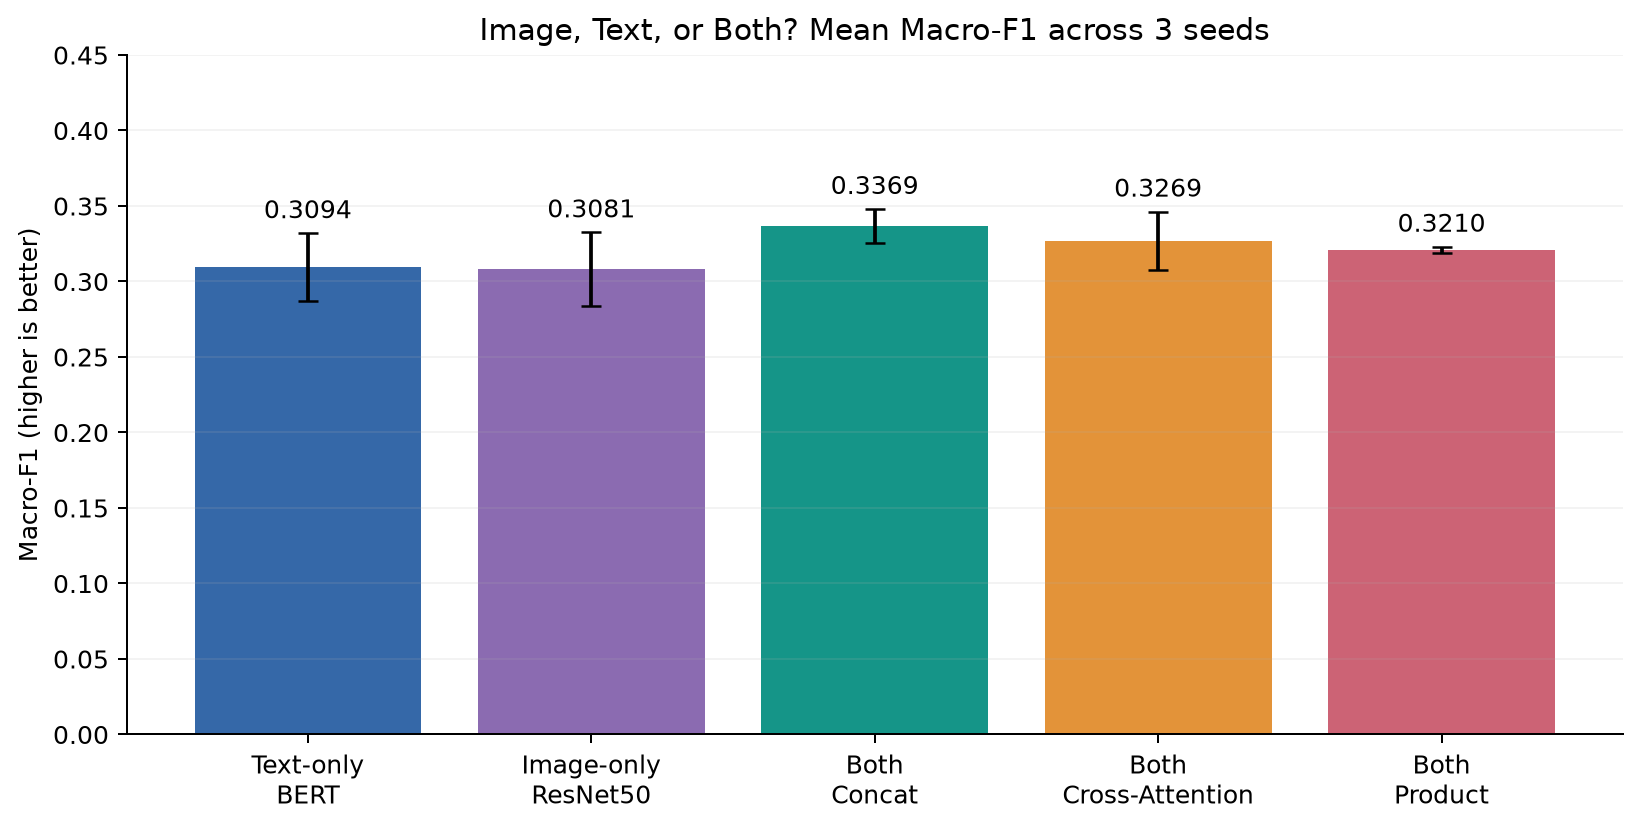
\includegraphics[width=0.88\linewidth]{figures/overall_performance.png}
\caption{Overall macro-F1 comparison from the saved analysis. Error bars describe run variation, not confidence intervals.}
\label{fig:overall}
\end{figure}

\subsection{Is the score improvement clear?}
Concatenation has the higher average score, but the statistical evidence is not strong enough to say it is clearly better. All six confidence intervals in Table~\ref{tab:paired} include zero, and all adjusted p-values are above 0.05. An interval containing zero means that no difference is still possible under this check. This does not prove the models are equal. We use concatenation as our main comparison model because of its observed score, not because its advantage is guaranteed.

\begin{table}[htbp]
\centering\small
\begin{tabular}{lrrr}
\toprule
Fusion vs. baseline & Gain (pp) & 95\% CI (pp) & Holm $p$ \\
\midrule
Concatenation vs. text & +2.75 & [-0.11, +5.62] & 0.3840 \\
Concatenation vs. image & +2.87 & [-0.83, +6.56] & 0.7112 \\
Cross-attention vs. text & +1.75 & [-0.78, +4.25] & 0.8288 \\
Cross-attention vs. image & +1.87 & [-1.48, +5.14] & 0.8288 \\
Product vs. text & +1.16 & [-1.68, +4.02] & 0.9027 \\
Product vs. image & +1.29 & [-2.38, +4.95] & 0.9027 \\
\bottomrule
\end{tabular}
\caption{Bootstrap ranges with fixed class counts and adjusted permutation-test p-values. CI means confidence interval; pp means percentage points.}
\label{tab:paired}
\end{table}

A separate check used 5,000 bootstrap samples without fixing class counts, with seed 20261006. Its concatenation-minus-text interval is $[-0.07,+5.68]$ points. The main check, using 20,000 samples with fixed class counts, gives $[-0.11,+5.62]$. The small difference comes from different sampling methods. Both include zero and support the same cautious conclusion. The main check supplies the statistical table; the separate check supplies extra group and duplicate-overlap results.

\subsection{Setup 2: Results by sentiment class}
Concatenation's largest gain is on neutral sentiment (Table~\ref{tab:class}), rising 10.41 F1 points above text and 8.26 points above images. Negative F1 improves slightly over text; positive F1 declines. A general claim that fusion improves every class would therefore be incorrect.

\begin{table}[htbp]
\centering\small
\begin{tabular}{lrrr}
\toprule
Model & Negative & Neutral & Positive \\
\midrule
Text (BERT) & 11.95 & 24.04 & 56.82 \\
Image (ResNet-50) & 7.50 & 26.18 & 58.77 \\
Concatenation & 13.49 & 34.45 & 53.11 \\
Cross-attention & 8.53 & 31.14 & 58.38 \\
Product & 12.08 & 33.90 & 50.31 \\
\bottomrule
\end{tabular}
\caption{Mean class F1 in percent; test class counts are 54 negative, 218 neutral, and 428 positive.}
\label{tab:class}
\end{table}

Recall shows how many true examples of a class the model finds. Average neutral recall rises from 26.61\% for text to 40.52\% for concatenation. Positive recall falls from 58.72\% to 47.04\%. Concatenation predicts neutral for about 183 positive memes per run, compared with about 125 for text. This helps explain why macro-F1 rises while accuracy falls. Negative F1 stays below 14\% for every model, so negative memes remain difficult even with class-weighted training.

Text seed 1 predicts positive for 680 of 700 memes, achieving 61.00\% accuracy but 28.34\% macro-F1. Cross-attention seed 2 reaches 52.86\% accuracy with zero negative-class F1. These observable patterns justify reporting class-level results alongside aggregate scores. Saved predictions establish the patterns but cannot identify their training-time cause.

\begin{figure}[htbp]
\centering
\begin{subfigure}{0.32\linewidth}\centering
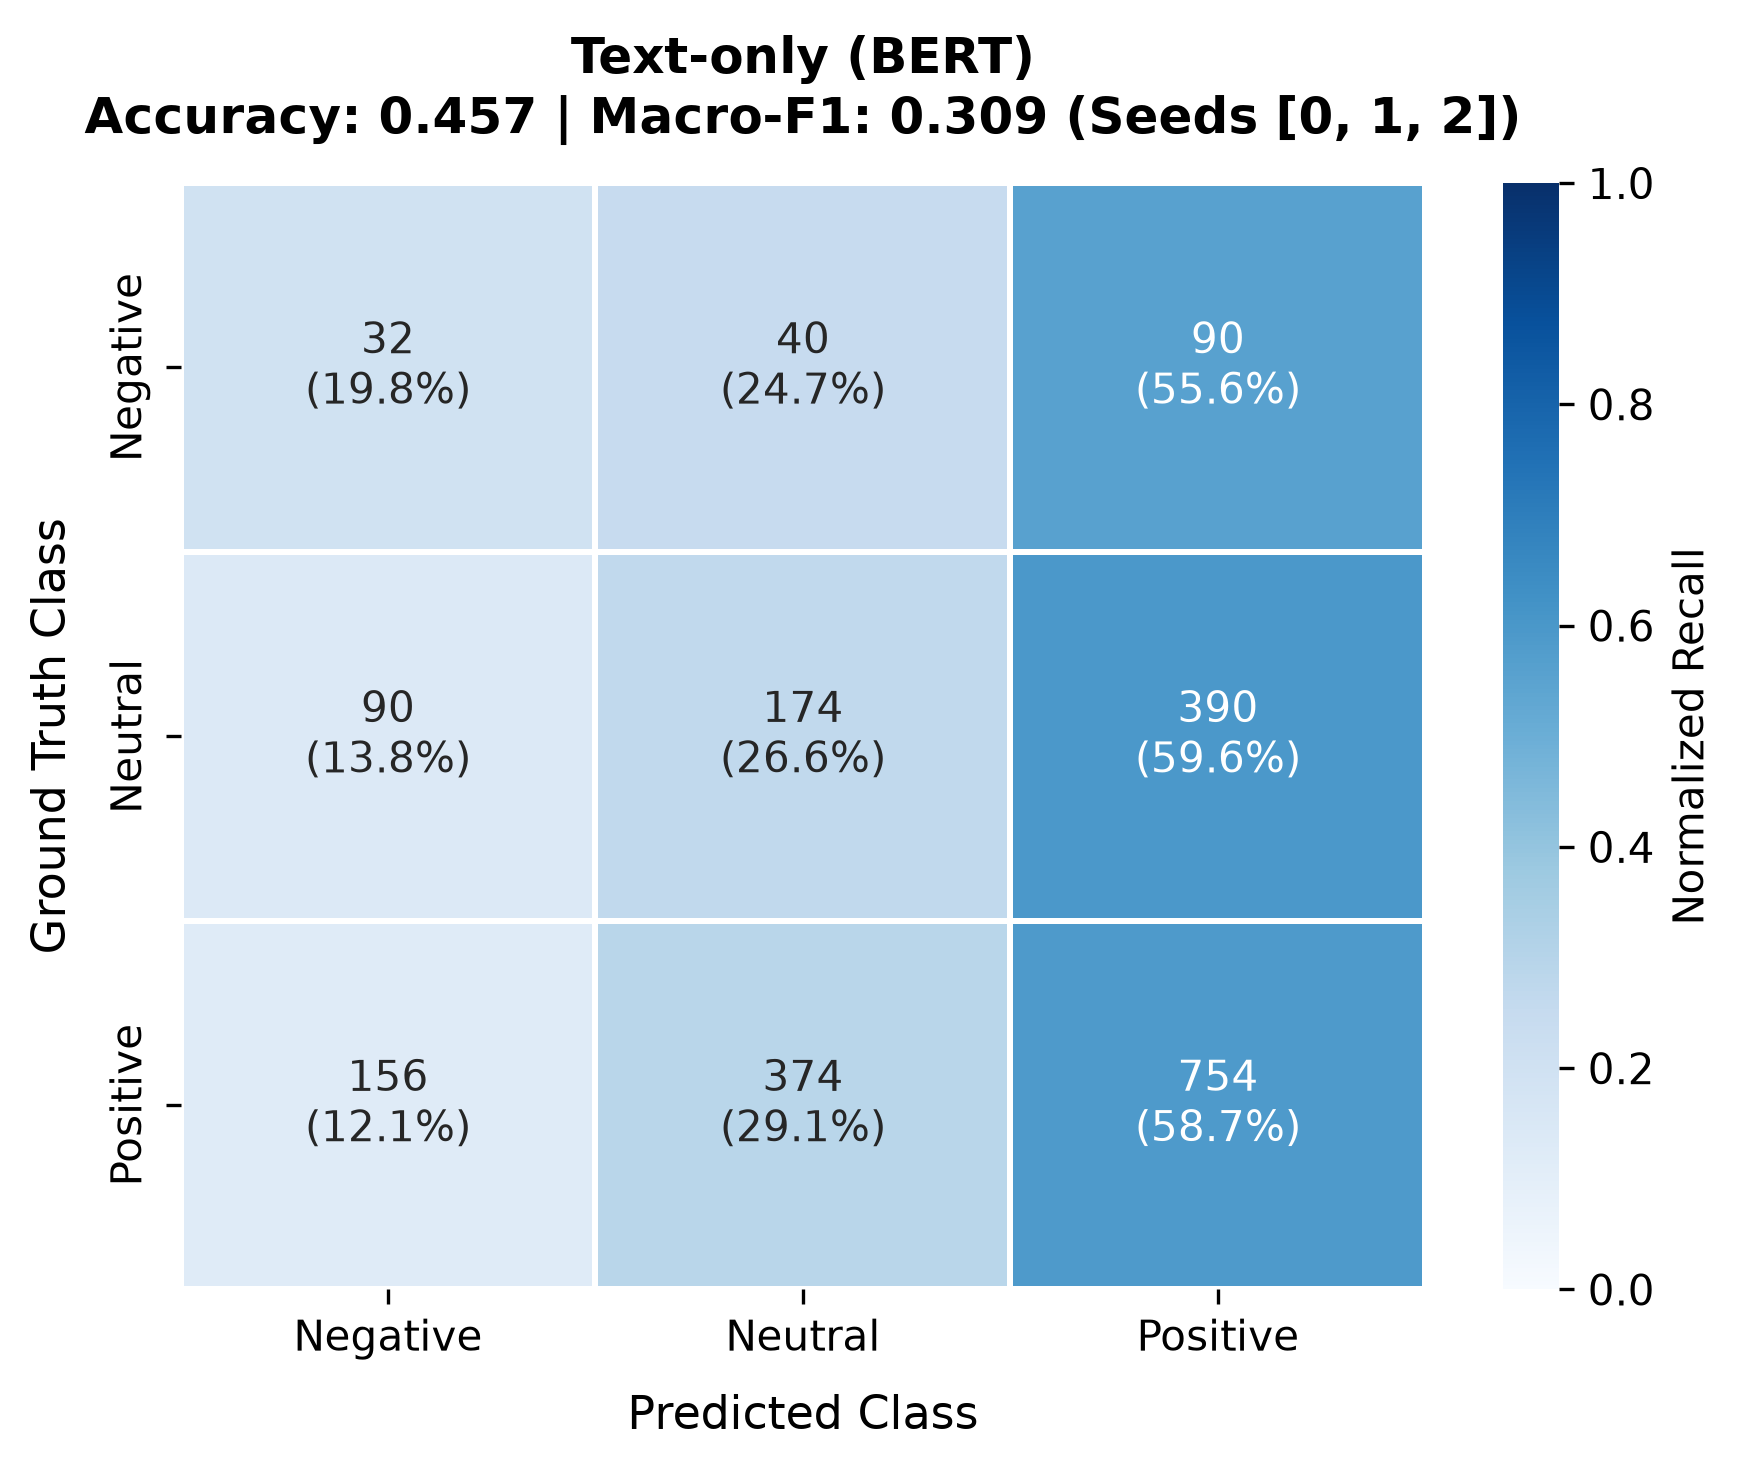
\includegraphics[width=\linewidth]{figures/cm_text.png}
\caption{Text}
\end{subfigure}\hfill
\begin{subfigure}{0.32\linewidth}\centering
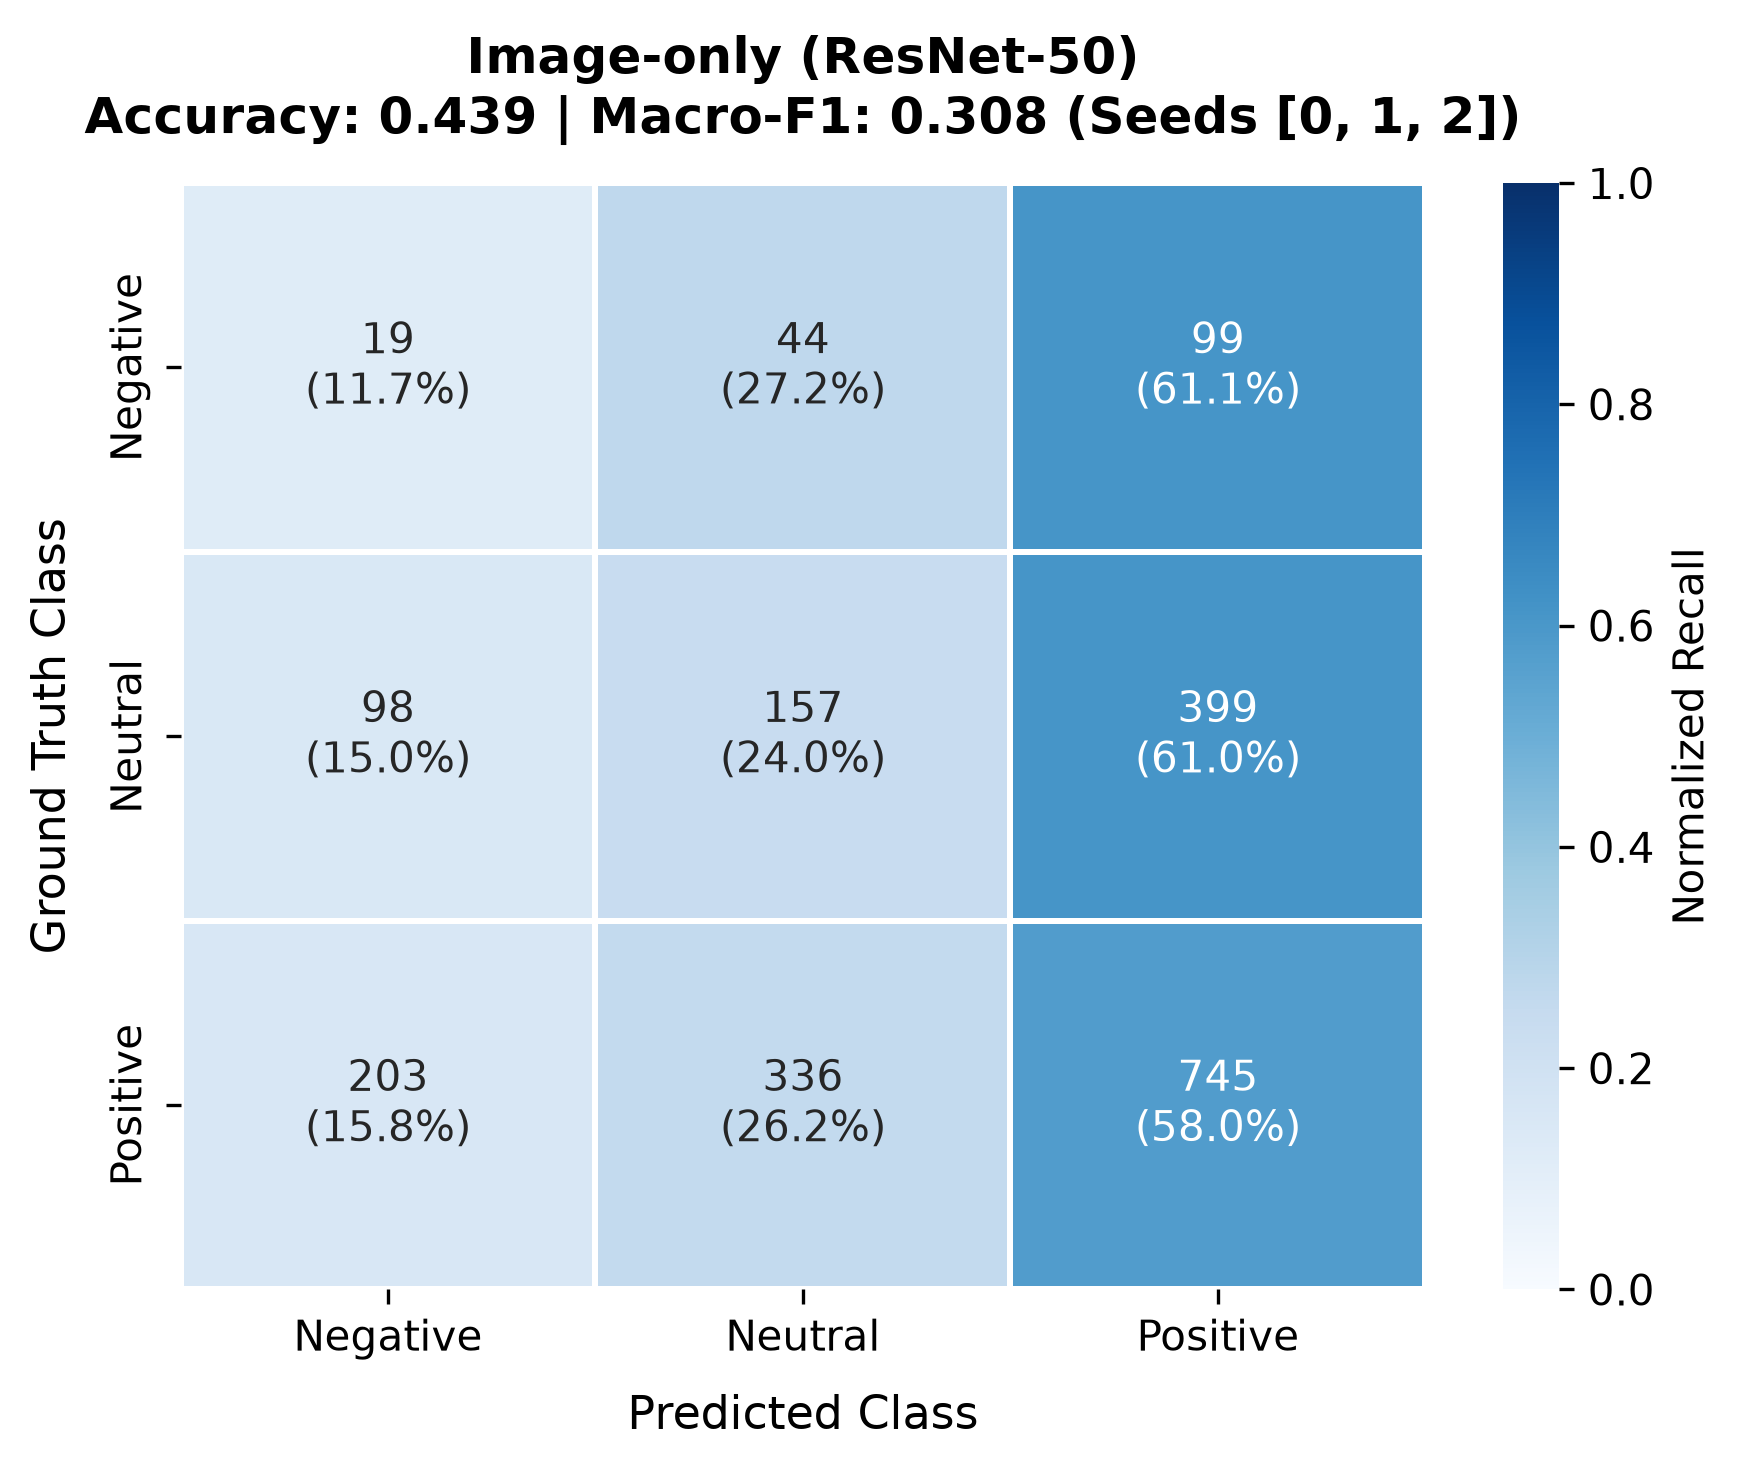
\includegraphics[width=\linewidth]{figures/cm_image.png}
\caption{Image}
\end{subfigure}\hfill
\begin{subfigure}{0.32\linewidth}\centering
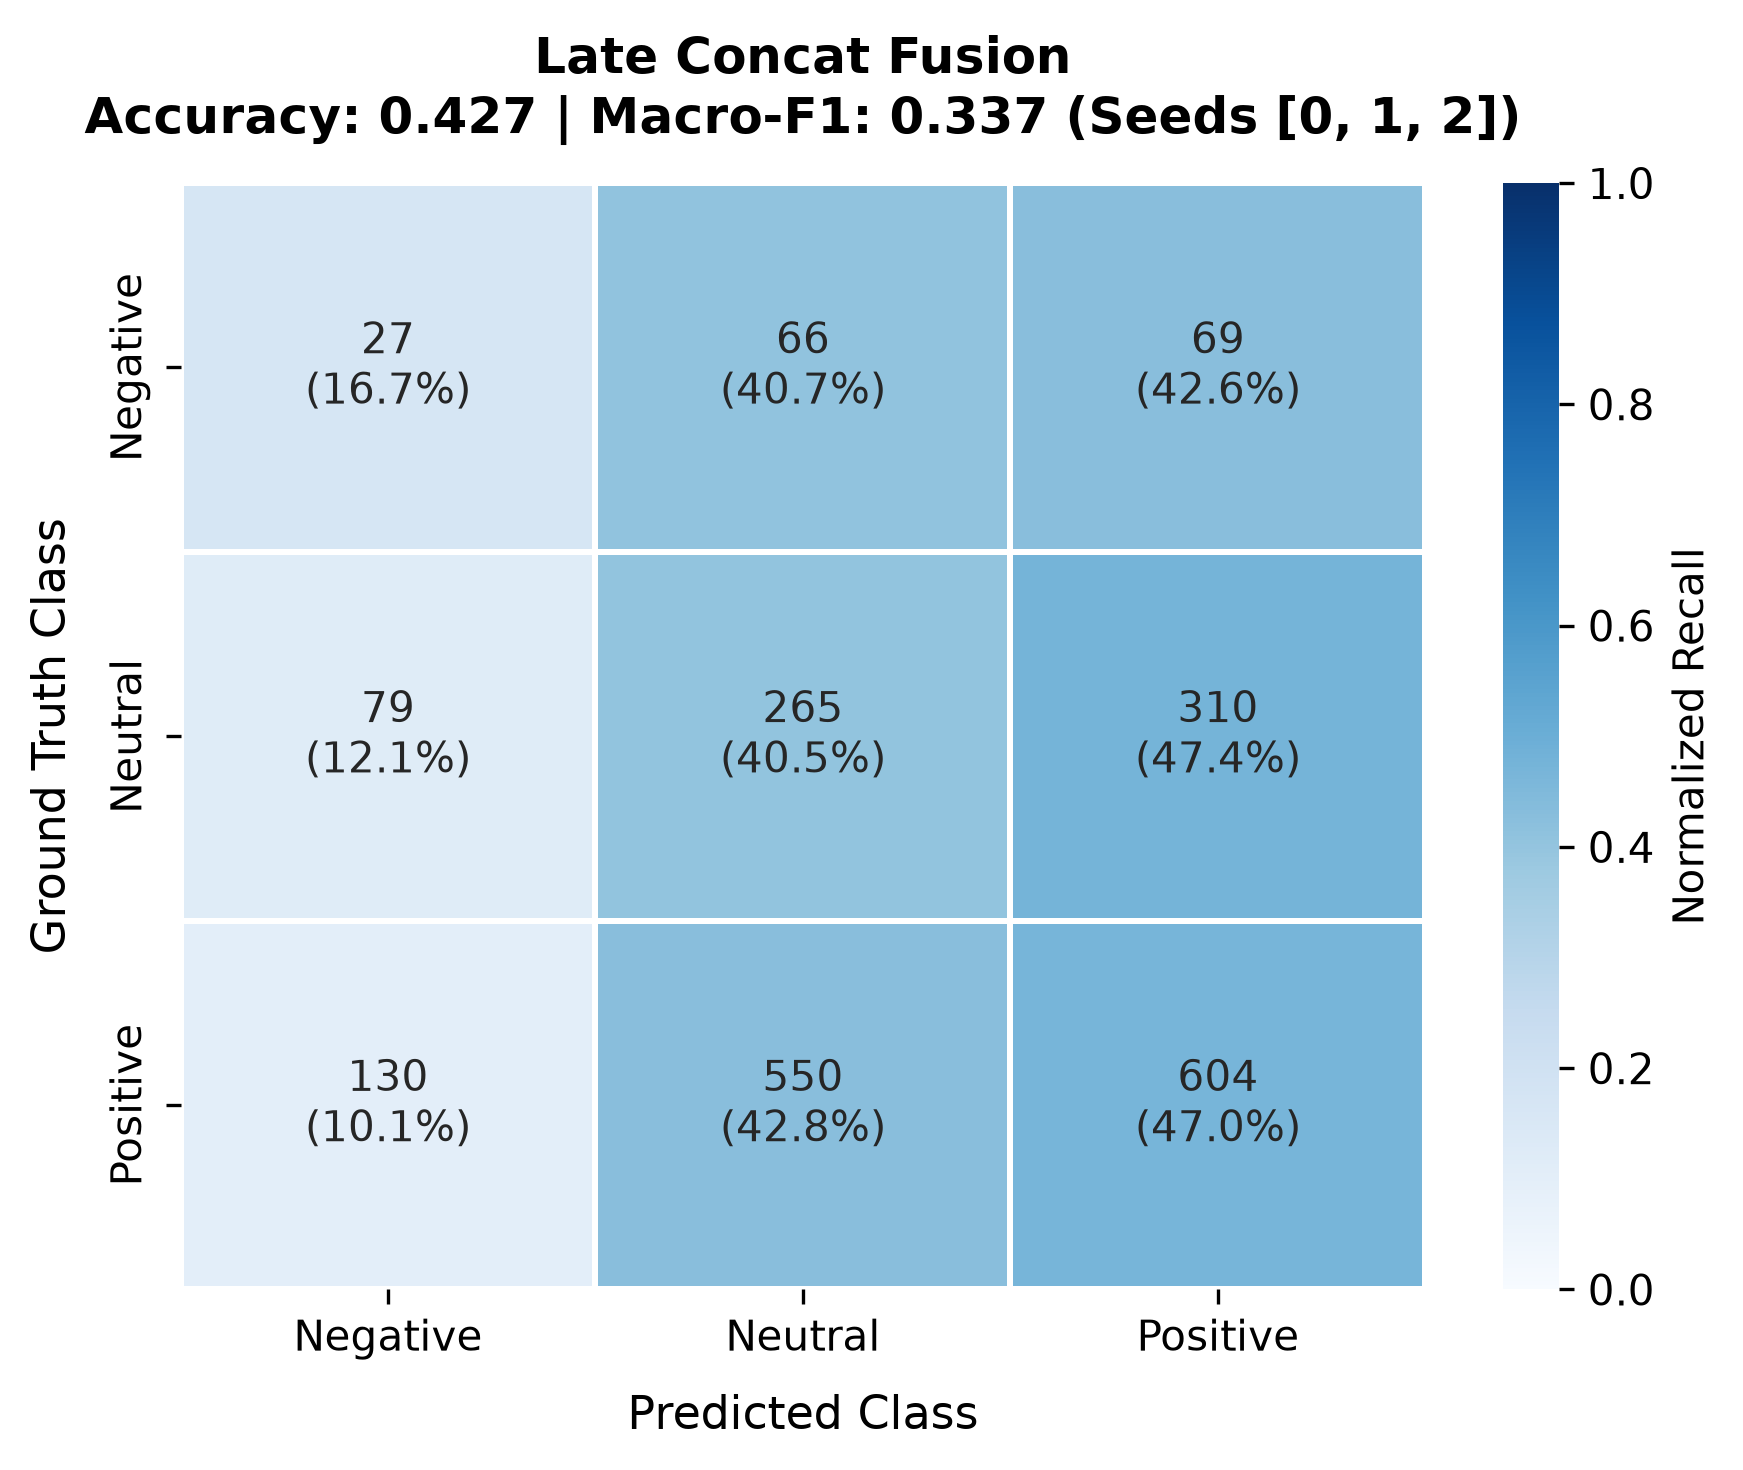
\includegraphics[width=\linewidth]{figures/cm_both_concat.png}
\caption{Concat}
\end{subfigure}\hfill
\par\medskip
\begin{subfigure}{0.32\linewidth}\centering
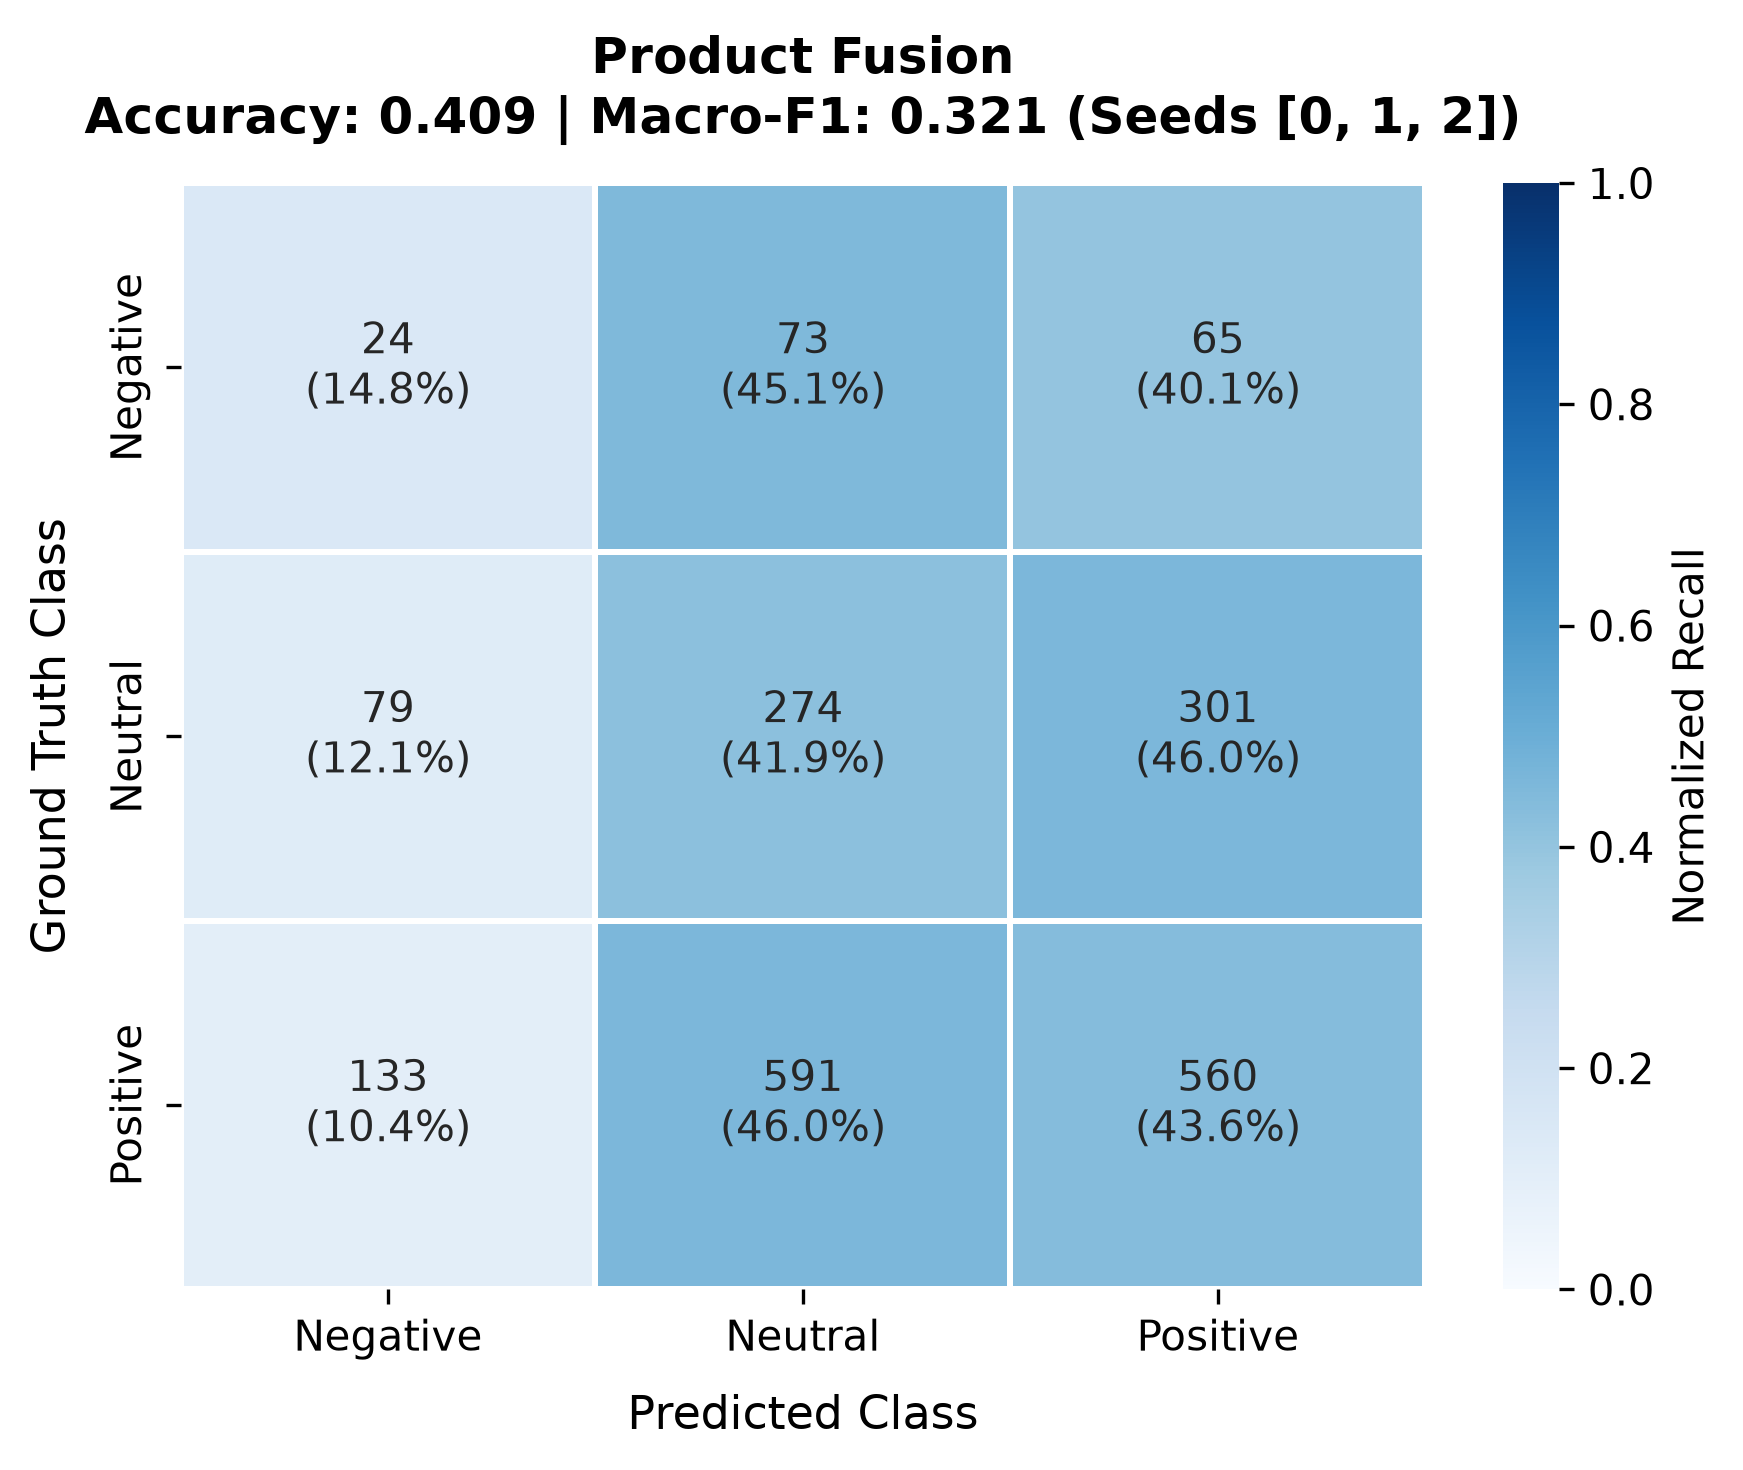
\includegraphics[width=\linewidth]{figures/cm_both_product.png}
\caption{Product}
\end{subfigure}\hfill
\begin{subfigure}{0.32\linewidth}\centering
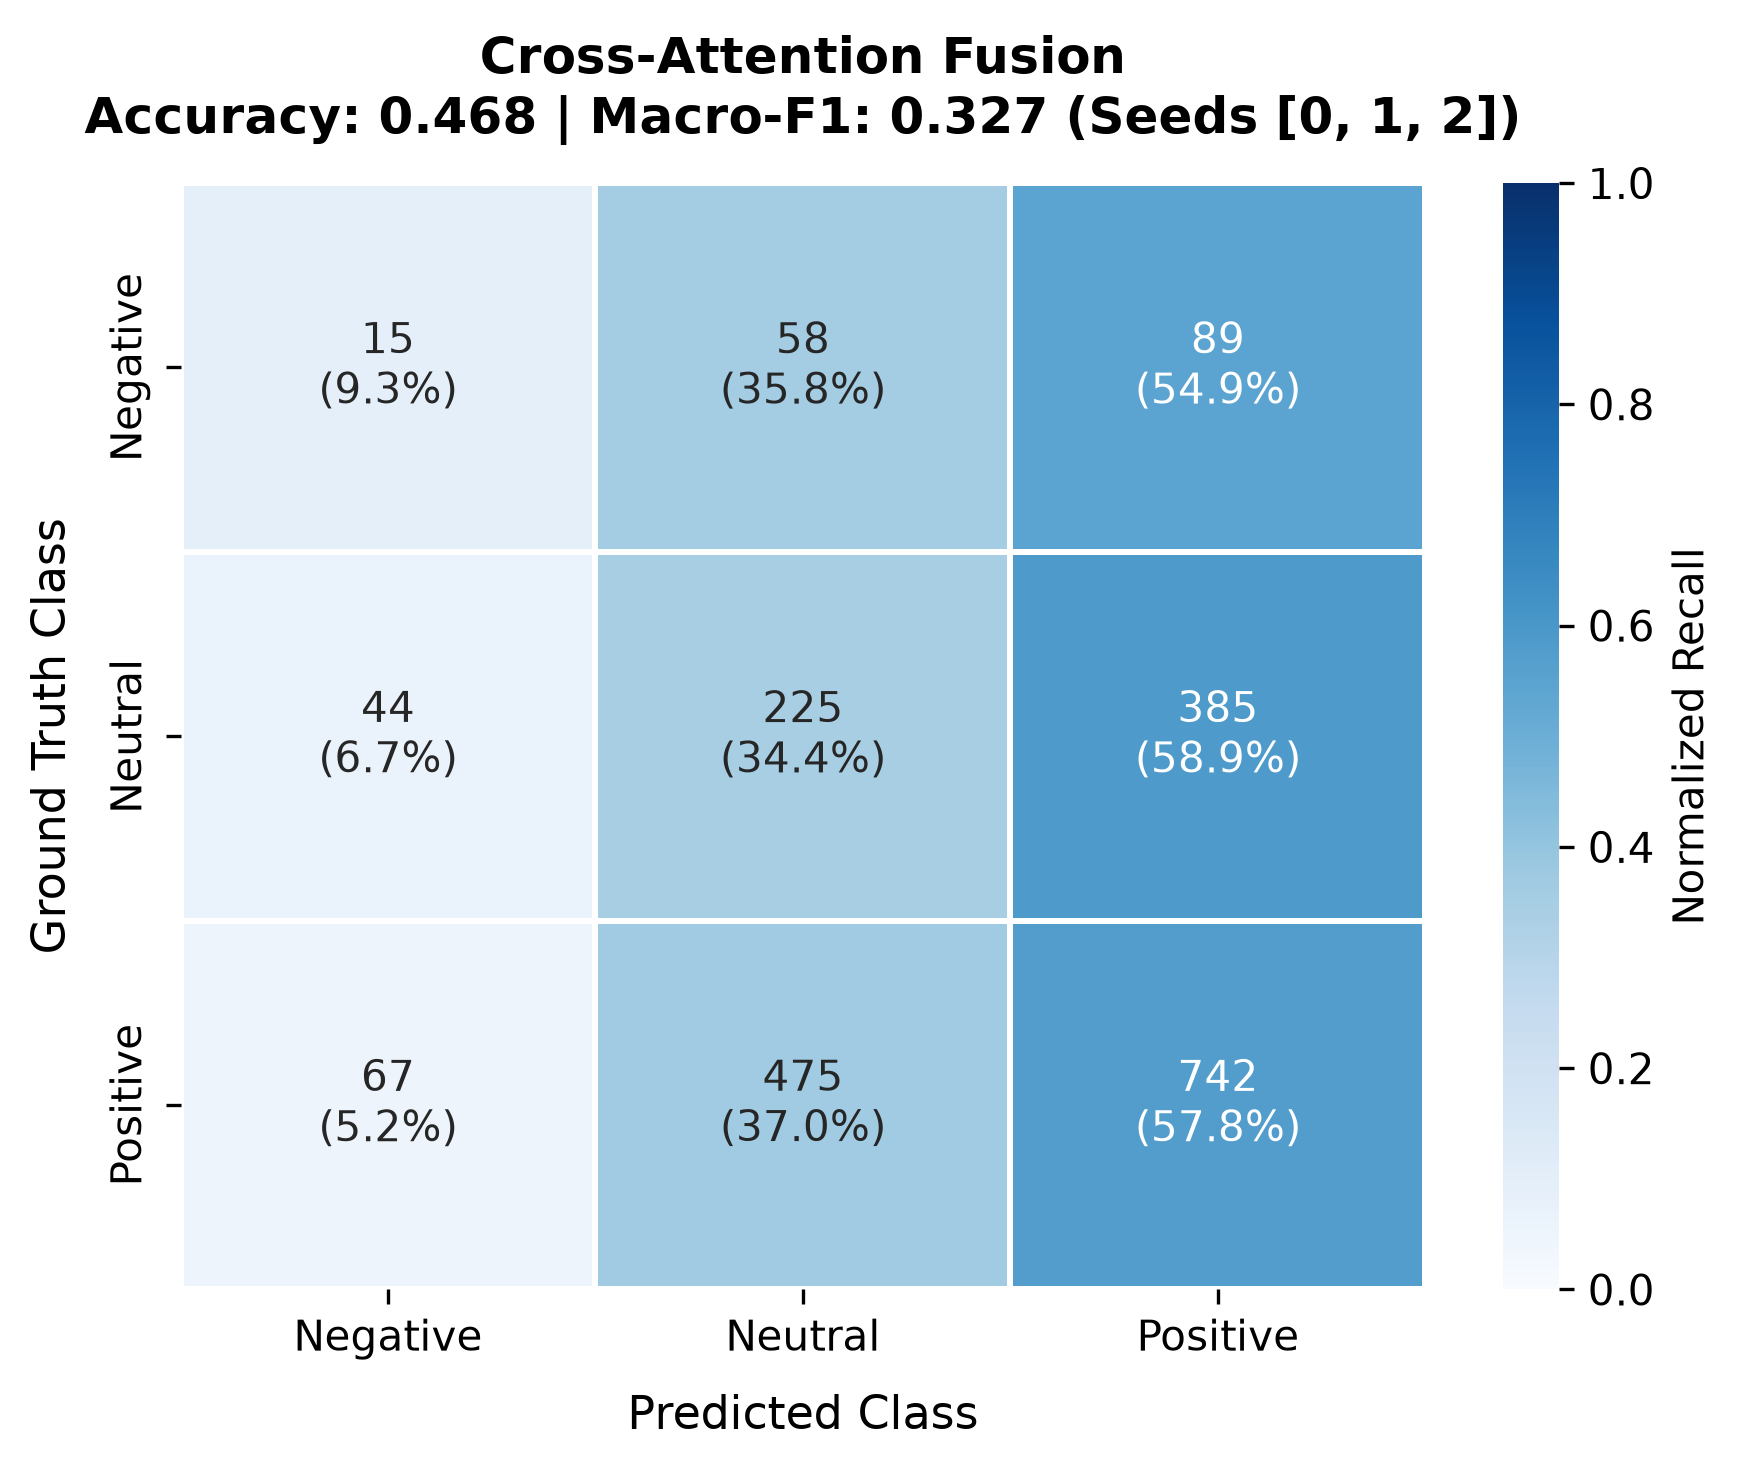
\includegraphics[width=\linewidth]{figures/cm_both_cross_attn.png}
\caption{Cross-attention}
\end{subfigure}\hfill
\caption{Prediction counts added across three runs, with percentages within each reference class. Rows are reference labels and columns are predictions. Each meme is counted three times; these are not 2,100 separate memes. Titles show average run scores.}
\label{fig:confusions}
\end{figure}

\subsection{Setup 2: Sarcasm, humor, and motivation}
We use the sarcasm, humor, and motivation labels to group memes, but still predict sentiment within each group. A group's score also depends on how many positive, neutral, and negative examples it contains. The same meme can appear in a sarcasm group and a humor group. Small groups have few negative examples. These tables describe our saved results; they do not prove that a model understands sarcasm or humor.

\begin{table}[htbp]
\centering\small
\begin{tabular}{lrrrrrr}
\toprule
Group & $n$ & Image & Text & Concat & Product & Attention \\
\midrule
Not sarcastic & 157 & 27.74 & 28.47 & 33.04 & 32.20 & 31.32 \\
Any sarcasm & 543 & 31.73 & 31.55 & 33.87 & 31.86 & 32.84 \\
General sarcasm & 343 & 33.71 & 29.01 & 31.63 & 29.25 & 33.25 \\
Twisted meaning & 151 & 26.72 & 35.03 & 34.74 & 35.38 & 30.51 \\
Very twisted & 49 & 34.16 & 36.19 & 38.52 & 31.13 & 31.35 \\
Not funny & 157 & 28.79 & 32.63 & 38.53 & 36.05 & 28.34 \\
Funny & 247 & 29.90 & 29.14 & 31.71 & 29.40 & 33.75 \\
Very funny & 238 & 29.22 & 30.55 & 32.10 & 31.12 & 31.76 \\
Hilarious & 58 & 37.10 & 29.02 & 27.20 & 30.04 & 33.46 \\
Motivational & 242 & 30.46 & 30.33 & 34.57 & 32.98 & 33.55 \\
Not motivational & 458 & 30.69 & 30.92 & 33.06 & 31.43 & 32.12 \\
\bottomrule
\end{tabular}
\caption{Mean subgroup sentiment macro-F1 in percent. Attention denotes cross-attention.}
\label{tab:groups}
\end{table}

Concatenation improves over text by 4.56 points on non-sarcastic memes and 2.31 points on sarcastic memes. The difference between these gains is $-2.25$ points, with a paired bootstrap interval of $[-8.77,+4.18]$. Thus there is no established special benefit for sarcasm. Within sarcasm, images lead on general sarcasm, product narrowly leads on twisted meaning, and concatenation leads on very twisted memes. The latter contains only 49 memes, including five negative examples.

The largest listed concatenation gain over text occurs on not-funny memes, at 5.90 points. Concatenation also gains 4.25 points on motivational memes. Images have the highest score on hilarious memes, where concatenation scores lower than both text-only and image-only. A stronger humor label therefore does not mean combining inputs will help. Cross-attention leads on the funny subgroup but does not lead in any listed sarcasm subgroup.

\begin{figure}[htbp]
\centering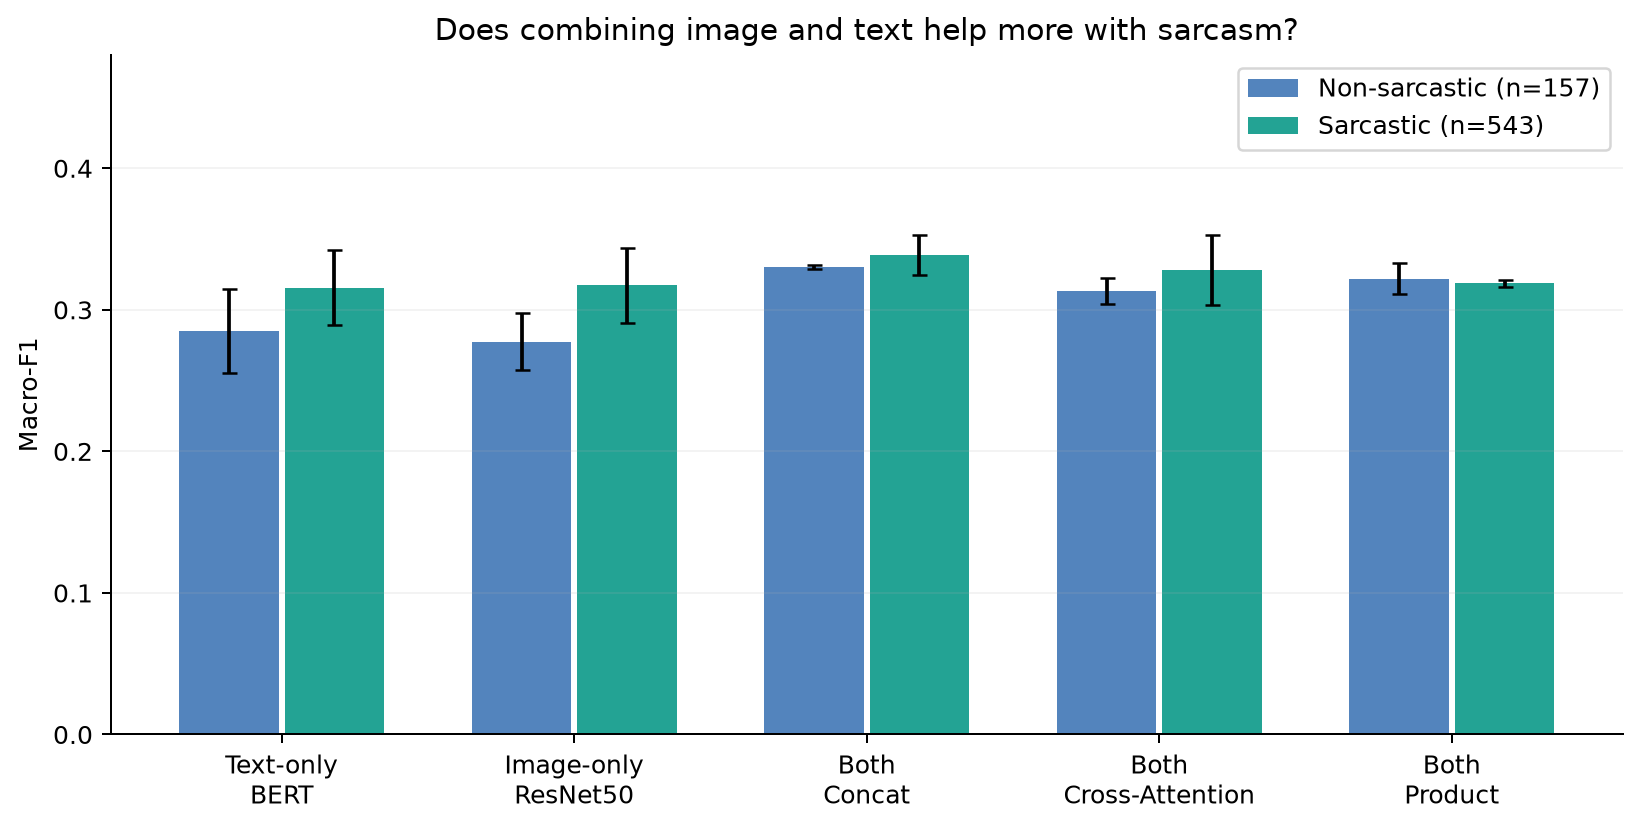
\includegraphics[width=0.85\linewidth]{figures/sarcasm_subgroups.png}
\caption{Sentiment macro-F1 on sarcastic and non-sarcastic memes. This is subgroup evaluation, not sarcasm detection.}
\label{fig:sarcasm}
\end{figure}

\subsection{Where each input helps or makes mistakes}
On average per run, text correctly labels 158.7 memes that images miss, while images correctly label 145.7 that text misses. Both are correct on 161.3 memes and both are wrong on 234.3. These averages add up to 700. This shows that each input helps on different examples. However, a combined model does not automatically keep all the successful decisions of both baselines.

Concatenation fixes 164, 102, and 138 text errors in seeds 0, 1, and 2, but introduces 144, 219, and 105 new errors. Nine specific memes are corrected in all three runs, while ten are made wrong in all three. Compared with images, these counts are 26 consistently corrected and 40 consistently made wrong. Counting correct answers helps explain accuracy, but macro-F1 also depends on which classes those answers belong to.

\subsection{Setup 3: Comparing the fusion methods}
Concatenation has the best observed macro-F1 with a simple joining operation. Product scores 1.59 points lower, and cross-attention scores 1.00 point lower. The statistical checks do not show a clear advantage between these methods. Attention can connect text features with image regions, but that does not prove it understands irony. We did not save speed or memory measurements, so we cannot say which model is faster or cheaper to run.

The best choice depends on the score we care about. Concatenation has higher macro-F1, while cross-attention has higher accuracy. All trained models still have lower average accuracy than always predicting positive. We chose the leading model after looking at these test results, so that choice is a finding for this test set rather than proof that it will lead on other data.

\subsection{Checking exact overlaps with training data}
The fit and holdout parts have no matching normalized captions or identical image files. Between training and test, ten test memes have matching captions and five have matching image files. Some match both, giving 11 test memes in total. Removing these without retraining leaves 689 test memes. Average macro-F1 becomes 30.94\% for images, 30.92\% for text, 33.81\% for concatenation, 32.21\% for product, and 32.65\% for cross-attention.

Concatenation stays first after removing these exact matches, so they do not explain its lead. The two baselines switch places by a tiny amount. This check does not find every similar image, reused template, or closely related caption. It also changes the test set rather than creating a new duplicate-free experiment. The holdout code keeps matching groups together but does not explicitly balance sentiment classes when shuffling them.

\section{Error and Qualitative Analysis}
\label{sec:error}

\subsection{Selection and interpretation}
We looked at 20 original meme images, their corrected captions, and their reference labels. The selection includes six cases where concatenation makes a correct text prediction wrong, six where it fixes a text error, and eight where all models are wrong. The selection favors confident concatenation predictions, so it is not a random sample. Tables~\ref{tab:cases} and~\ref{tab:cases-cont} describe the content and possible reasons for errors. These reasons are explanations to consider, not proven causes.

For these two tables only, we average each model's probabilities across its three runs and choose the class with the highest average. This gives one combined prediction per model, often called an ensemble prediction. It differs from the per-run scoring used in the results tables. A wrong combined prediction does not mean all three runs were wrong. \textbf{N = negative, U = neutral, and P = positive.} Predictions are listed in the order \textbf{text / image / concat / attention / product}. The reference label, also called the gold label, is the dataset's answer. It is not a new judgment made by our group. Every listed case contains at least one model error.

\setlength{\tabcolsep}{4pt}
\small
\clearpage
\begin{table}[p]
\centering\small
\begin{tabular}{>{\raggedright\arraybackslash}p{1.95cm}>{\raggedright\arraybackslash}p{2.30cm}>{\raggedright\arraybackslash}p{2.1cm}>{\raggedright\arraybackslash}p{7.1cm}}
\toprule
ID & Content category & Reference; predictions & Observation and possible explanation \\
\midrule
\texttt{test\_00239} & Threat and template tone & U; U/N/N/P/N & A familiar portrait appears beside a threat. Text correctly predicts neutral; concat predicts negative. The threatening words and familiar template may suggest different feelings. \\[4pt]
\texttt{test\_00343} & Encouraging message & P; P/U/U/U/U & A woman exercising appears beside an encouraging message. Text correctly predicts positive; all three combined models predict neutral. Adding the image changes a correct answer into a mistake. \\[4pt]
\texttt{test\_00662} & Wordplay and reference & P; P/P/U/U/U & A TV character appears beside a cow-and-cliff pun using ledge, legend, and dairy. Text and image models correctly predict positive; all three combined models predict neutral. \\[4pt]
\texttt{test\_00597} & Mixed feelings & P; P/P/U/U/P & A serious portrait appears beside a message about surviving hardship. Text and images correctly predict positive; concat and attention predict neutral. The message includes both encouragement and painful experiences. \\[4pt]
\texttt{test\_00221} & Fictional character & P; P/U/U/U/U & A Joker portrait appears beside a question about waking up as him. The reference label is positive. Text matches it, while the combined models predict neutral. The character and overall tone may suggest different feelings. \\[4pt]
\texttt{test\_00045} & Social joke and text error & P; P/P/U/U/U & A smiling portrait appears beside a joke about trying to stay relevant. ABOUTA is merged in the caption. Both baselines correctly predict positive; combined models predict neutral. The effect of the text error was not tested. \\[4pt]
\texttt{test\_00194} & Dark humor & P; N/P/P/P/P & A made-up technology headline jokes about reviving a historical figure linked to atrocities. Text predicts negative; images and combined models match positive. A positive sentiment label does not mean the content is harmless. \\[4pt]
\texttt{test\_00043} & Ironic prayer & U; P/P/U/U/U & A praying character gives thanks for a girlfriend. Text predicts positive; concat correctly predicts neutral. The scene may help, but concat also predicts neutral more often overall. \\[4pt]
\texttt{test\_00506} & Image expression & P; U/P/P/P/P & A triumphant child appears beside a short remark about a tall person. Text predicts neutral; images and combined models correctly predict positive. The facial expression may add information missing from the short caption. \\[4pt]
\texttt{test\_00292} & Everyday joke and film scene & P; N/N/P/P/P & A dramatic film scene accompanies forgetting a phone while using the toilet. Both baselines predict negative; all combined models correctly predict positive. The contrast may explain the joke, but we did not test how the model uses it. \\[4pt]
\bottomrule
\end{tabular}
\caption{Inspected cases 1--10: errors introduced by fusion and corrected baseline errors.}
\label{tab:cases}
\end{table}
\begin{table}[p]
\centering\small
\begin{tabular}{>{\raggedright\arraybackslash}p{1.95cm}>{\raggedright\arraybackslash}p{2.30cm}>{\raggedright\arraybackslash}p{2.1cm}>{\raggedright\arraybackslash}p{7.1cm}}
\toprule
ID & Content category & Reference; predictions & Observation and possible explanation \\
\midrule
\texttt{test\_00228} & Character catchphrase & P; U/P/P/U/P & A cartoon body with a changed face uses an authoritarian catchphrase. Text and attention predict neutral; images, concat, and product correctly predict positive. Different fusion methods do not always fix the same error. \\[4pt]
\texttt{test\_00344} & Dialogue and picture layout & U; P/U/U/P/U & Two cooking-show panels show bread framing a face during an insult. Text and attention predict positive; images, concat, and product correctly predict neutral. The speakers and scene make the overall tone harder to judge. \\[4pt]
\texttt{test\_00423} & Sad words and extra tags & U; N/N/N/N/N & A sad frog appears beside a complaint about eating and unhappiness, followed by many tags. Every model predicts negative, but the reference is neutral. Literal sadness and the familiar joke may suggest different readings. \\[4pt]
\texttt{test\_00557} & Offensive content & U; N/N/N/P/N & A photo appears beside a racist slavery joke. Four models predict negative and attention predicts positive, but the reference is neutral. Offensive content and overall sentiment are different properties. \\[4pt]
\texttt{test\_00091} & Fan reference & P; N/N/N/N/N & A fictional character appears beside a statement about people who like him. Every model predicts negative, but the reference is positive. Recognizing a fan's positive message may require knowledge of the character. \\[4pt]
\texttt{test\_00233} & Political joke & U; N/P/N/N/N & A political leader appears beside a claim about legalizing pizza. Every model misses neutral. The unusual claim and views about the leader may suggest different feelings. \\[4pt]
\texttt{test\_00424} & Short caption and template & U; N/P/N/P/P & A sad frog appears against bright colors with only its template name. Every model misses neutral. The text gives little sentiment information, while the face and background may suggest different feelings. \\[4pt]
\texttt{test\_00695} & Promotional message & U; P/P/P/P/P & A text-heavy post links celebrations to a digestive product. Every model predicts positive, but the reference is neutral. Cheerful wording may hide the mainly informational or promotional purpose. \\[4pt]
\texttt{test\_00148} & Visual resemblance & U; P/P/N/P/P & A celebrity and film character are shown side by side because they look alike. Concat predicts negative and the other models positive, but the reference is neutral. Recognizing resemblance does not settle the sentiment. \\[4pt]
\texttt{test\_00085} & Fictional plot & P; U/U/U/U/U & A fictional character appears beside a story about attraction and betrayal. Every model predicts neutral, but the reference is positive. The actions, story reference, and joke may lead to different judgments. \\[4pt]
\bottomrule
\end{tabular}
\caption{Inspected cases 11--20: additional corrected errors and shared ensemble failures.}
\label{tab:cases-cont}
\end{table}
\clearpage

\normalsize
\setlength{\tabcolsep}{6pt}

\subsection{Recurring patterns}
\paragraph{Fusion can introduce repeatable mistakes.}
The exercise poster, survival quote, and cow pun are correctly labeled positive by the text model's combined prediction, but concatenation changes them to neutral. This matches the overall pattern of more positive-to-neutral mistakes. It does not show which image feature caused the change. In the threat portrait, text correctly predicts neutral and concatenation predicts negative. The threatening words and the familiar template may suggest different readings.

\paragraph{Images can help correct text errors.}
Fusion corrects the text error on the triumphant child, forgotten-phone joke, and prayer scene. The image may add useful context, but a correct answer does not tell us how the model got there. It could use a familiar template or a common class rather than connect the caption and image meaning. The catchphrase and cooking-show examples also show that a correction by concatenation is not always a correction by attention.

\paragraph{References and labels can be difficult.}
All models' combined predictions miss the reference label on the fandom statement, political pizza joke, celebrity comparison, and fictional betrayal scene. Understanding these examples may depend on a character, a reference, or the audience's reaction. The racist joke also shows why sentiment and offensiveness are different: a neutral sentiment label does not mean the content is acceptable. Without independently checking the labels again, we cannot fully separate model mistakes from reasonable disagreement with a subjective label.

\paragraph{Text quality is not fully resolved.}
Some corrected captions still contain merged words, website names, or long lists of tags. These may make prediction harder, but we did not compare cleaned captions with the originals. We cannot say that OCR errors caused a particular mistake. Our models receive corrected captions; they are not being tested on automatically reading all text from the image.

\begin{figure}[htbp]
\centering
\begin{subfigure}{0.23\linewidth}\centering
\includegraphics[width=\linewidth,height=4cm,keepaspectratio]{../data/memotion/img/test_00343.png}
\caption{Motivational poster}
\end{subfigure}\hfill
\begin{subfigure}{0.23\linewidth}\centering
\includegraphics[width=\linewidth,height=4cm,keepaspectratio]{../data/memotion/img/test_00043.png}
\caption{Prayer scene}
\end{subfigure}\hfill
\begin{subfigure}{0.23\linewidth}\centering
\includegraphics[width=\linewidth,height=4cm,keepaspectratio]{../data/memotion/img/test_00292.png}
\caption{Dramatic mismatch}
\end{subfigure}\hfill
\begin{subfigure}{0.23\linewidth}\centering
\includegraphics[width=\linewidth,height=4cm,keepaspectratio]{../data/memotion/img/test_00148.png}
\caption{Visual comparison}
\end{subfigure}
\caption{Original examples illustrating a new fusion error, two corrected baseline errors, and a shared ensemble failure. Their prediction labels and interpretations are recorded in Tables~\ref{tab:cases} and~\ref{tab:cases-cont}.}
\label{fig:cases}
\end{figure}

\subsection{What this analysis cannot show}
We did not have attention maps or saved checkpoints for experiments that hide or replace an input. We therefore cannot show which image region or phrase caused a prediction. The examples help describe model behavior, but their selected counts do not tell us how common each problem is. They also do not prove that a correct answer depends on matching the image with its caption.

\clearpage
\section{Conclusion and Limitations}
\label{sec:conclusion}

Image-only and text-only have almost the same average macro-F1, and the better model changes across seeds. Each gets some examples right that the other misses (RQ1). All three combined models have higher average macro-F1, with concatenation leading at 33.69\%. However, the statistical checks do not provide enough evidence for a clear fusion advantage (RQ2). Concatenation finds more neutral memes but misses more positive ones, so fusion mainly shifts predictions toward neutral rather than giving a clear overall gain. Gains vary between meme groups, and there is no proven special advantage for sarcasm (RQ3).

This project predicts sentiment, which is only one part of understanding a meme. Images still contain printed words, captions can have mistakes, and sentiment labels depend on people's judgments. Only 54 test memes are negative. Training and feature processing also differ between models (for example, text-only uses BERT pooler output while fusion uses first-token features), so gains cannot be attributed to fusion alone. Subgroup results in Table 6 are descriptive only: groups are small and have no confidence intervals or multiple-comparison control. We have three seeds and incomplete training records, which limits claims about repeatability. Removing exact overlaps does not remove every similar template. Our local split also differs from the competition split, so the scores are not leaderboard comparisons.

Our main finding is that text and images help on different examples; simple concatenation gives the highest observed macro-F1, but the gain is not statistically clear. Its improvement is modest and uneven. The results do not prove that combining inputs is always better or that the models fully understand the joke.

\clearpage
\begin{thebibliography}{99}

\bibitem{sharma2020semeval}
C.~Sharma, D.~Bhageria, W.~Scott, S.~PYKL, A.~Das, T.~Chakraborty, V.~Pulabaigari, and B.~Gamb\"ack,
\newblock ``SemEval-2020 Task 8: Memotion Analysis--The Visuo-Lingual Metaphor!,''
\newblock in \emph{Proceedings of the Fourteenth Workshop on Semantic Evaluation}, pp.~759--773, 2020.
\newblock \href{https://aclanthology.org/2020.semeval-1.99/}{Primary source}.

\bibitem{devlin2019bert}
J.~Devlin, M.-W.~Chang, K.~Lee, and K.~Toutanova,
\newblock ``BERT: Pre-training of Deep Bidirectional Transformers for Language Understanding,''
\newblock in \emph{Proceedings of NAACL-HLT}, pp.~4171--4186, 2019.
\newblock \href{https://aclanthology.org/N19-1423/}{Primary source}.

\bibitem{he2016deep}
K.~He, X.~Zhang, S.~Ren, and J.~Sun,
\newblock ``Deep Residual Learning for Image Recognition,''
\newblock in \emph{Proceedings of the IEEE Conference on Computer Vision and Pattern Recognition (CVPR)}, pp.~770--778, 2016.
\newblock \href{https://openaccess.thecvf.com/content_cvpr_2016/html/He_Deep_Residual_Learning_CVPR_2016_paper.html}{Primary source}.

\bibitem{vaswani2017attention}
A.~Vaswani, N.~Shazeer, N.~Parmar, J.~Uszkoreit, L.~Jones, A.~N.~Gomez, \L.~Kaiser, and I.~Polosukhin,
\newblock ``Attention Is All You Need,''
\newblock in \emph{Advances in Neural Information Processing Systems (NeurIPS)}, pp.~5998--6008, 2017.
\newblock \href{https://arxiv.org/abs/1706.03762}{Primary source}.

\bibitem{bonheme2020sesam}
L.~Bonheme and M.~Grzes,
\newblock ``SESAM at SemEval-2020 Task 8: Investigating the Relationship between Image and Text in Sentiment Analysis of Memes,''
\newblock in \emph{Proceedings of the Fourteenth Workshop on Semantic Evaluation}, pp.~804--816, 2020.
\newblock \href{https://aclanthology.org/2020.semeval-1.102/}{Primary source}.

\bibitem{zadeh2017tensor}
A.~Zadeh, M.~Chen, S.~Poria, E.~Cambria, and L.-P.~Morency,
\newblock ``Tensor Fusion Network for Multimodal Sentiment Analysis,''
\newblock in \emph{Proceedings of the 2017 Conference on Empirical Methods in Natural Language Processing (EMNLP)}, pp.~1103--1114, 2017.
\newblock \href{https://aclanthology.org/D17-1115/}{Primary source}.

\end{thebibliography}

\clearpage
\appendix
\section{Member Contributions}
\label{sec:appendix}

\begin{table}[h]
\centering
\small
\begin{tabular}{>{\raggedright\arraybackslash}p{4.2cm}l>{\raggedright\arraybackslash}p{8cm}}
\toprule
\textbf{Member} & \textbf{Student ID} & \textbf{Contribution} \\
\midrule
Nguyen Tuan Vinh & 2411040 & Implemented and trained concatenation and product fusion models using BERT and ResNet-50 features. \\
Nguyen Dinh Phu Vinh & 2411042 & Implemented and trained text-to-image cross-attention with spatial image features. \\
Nguyen Dang Dat & 2411117 & Prepared data, normalized labels, verified images, organized splits, and wrote the report. \\
Duong Minh Duc & 2411136 & Computed metrics, statistical comparisons, subgroup results, error analyses, and visualizations. \\
Do Minh Tan & 2411032 & Implemented, trained, and evaluated the BERT text-only baseline across three seeds. \\
Vu Hoang Phuong & 2410808 & Implemented, fine-tuned, and evaluated the ResNet-50 image-only baseline across three seeds. \\
\bottomrule
\end{tabular}
\caption{Member contributions and student IDs.}
\label{tab:contributions}
\end{table}


\end{document}

